
\documentclass[12pt,a4paper,landscape]{article}
\usepackage[latin1]{inputenc}
\usepackage{amsmath}
\usepackage{amsfonts}
\usepackage{amssymb}
\usepackage{graphicx}
\usepackage{lscape}
\usepackage{multicol}
\usepackage{setspace}
\usepackage[margin=2.5cm]{geometry}
\newcommand{\est}[2]{\begin{array}[t]{c}
\hspace{-.125in}#1\hspace{-.125in}\vspace{-.13in}\\ 
\hspace{-.125in}#2\hspace{-.125in}
\end{array}}
\linespread{1.6}
\newcommand{\maa}{ (\mathsf{1}   - \est{\mathsf{  0.70}}{(\mathsf{  0.06})} B^{\mathsf{12}} ) }
\newcommand{\nrdiff}{\nabla} 
\newcommand{\nadiff}{\nabla_{\mathsf{12}}}
\newcommand{\ifadf}{ }
\begin{document}
\begin{flushleft}
\thispagestyle{empty}
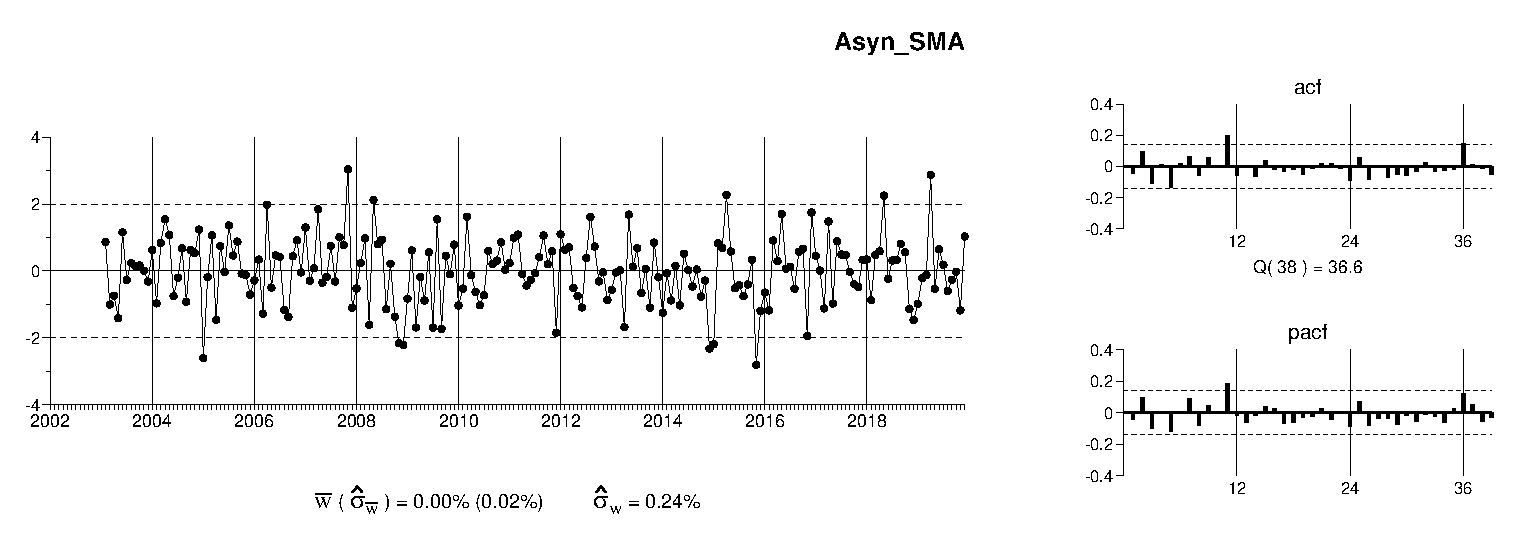
\includegraphics[scale=1]{Asyn_SMA.eps}
\begin{footnotesize}
 $ \nrdiff 
\nadiff 
\ifadf \ln \mathsf{IPCM}_{t} = \maa 
\mathsf{Asyn_SMA_{t}} ; \quad 
\hat{\sigma}_{\mathsf{Asyn_SMA}}=  \mathsf{ 0.25 } \%  $ 

\bigskip 
\begin{multicols}{2}{ 
\begin{tabular}{ccc}
\hline  Obs.  &  Date &  Std. Val. \\ 
\hline 
                       58 &       11/2007 &          3.04 \vspace{-.12in} \\  
 \end{tabular} 
\\ 
 \columnbreak 
 \singlespacing 
 \underline{\textbf{Comments:}} \\ 
 \bigskip       

% \underline{Action:} 
 } 
\end{multicols} 

\end{footnotesize}
\end{flushleft}
\end{document}
